\documentclass[12pt]{article}
\usepackage[utf8]{inputenc}
\usepackage{amsmath}
\usepackage{amssymb}
\usepackage{graphicx}
\usepackage{pgfplots}
\usepackage[margin=1in]{geometry}
\newcommand{\x}{\cdot}
\newcommand{\eval}[3]{\left.#1\right\rvert_{#2}^{#3}}
\newcommand{\nroot}[2]{\sqrt[\leftroot{-1}\uproot{1}#1]{#2}}
\newcommand{\paren}[1]{\left(#1\right)}
\newcommand{\braks}[1]{\left[#1\right]}
\newcommand{\curly}[1]{\left\{#1\right\}}
\newcommand{\norm}[1]{\lVert#1\rVert}
\newcommand{\inner}[2]{\langle#1,#2\rangle}
\newcommand{\argmax}[1]{\underset{#1}{\operatorname{arg\,max\,}}}
\newcommand{\argmin}[1]{\underset{#1}{\operatorname{arg\,min\,}}}

\tikzset{
	jumpdot/.style={mark=*,solid},
	excl/.append style={jumpdot,fill=white},
	incl/.append style={jumpdot,fill=blue},
}

\begin{document}

\begin{center}
	\LARGE{Decision Trees}
\end{center}

\section{Hypothesis}

Consider the domain $\mathcal{X} = \mathbb{R}^D$ and the codomain  $\mathcal{Y} =[1, M]$. In Decision Tree based classification, our hypothesis $h_\theta : \mathcal{X} \rightarrow \mathcal{Y}$ is defined by a (almost always binary) tree which partitions the feature space into regions with consistent labels. Inner nodes of the tree consist of decisions, which partition the data based on some threshold of some feature. Each leaf represents a label with which the data point will be classified.

\section{Decisions}

For each subset of data, we choose the split that minimizes the ``cost" of the two new subsets. To choose a split, we check all features and all thresholds for each (which are the values in the data points themselves). Thus, we have
\[ (f^*, t^*) = \arg\min\limits_{f\in[1,M]}\min\limits_{t\in\mathcal{T}_f}\text{cost}(S_l) + \text{cost}(S_r) \]
\vspace*{-1em}
\[ \mathcal{T}_f = \{x^{(f)}_i : \forall\mathbf{x}_i \in S \} \]
\[ S_l = \{(\mathbf{x}_i, y_i) : x^{(f)}_i \leq t \} \]
\[ S_r = \{(\mathbf{x}_i, y_i) : x^{(f)}_i > t \} \]
In other words, $\mathcal{T}_f$ are all values of a feature $f$, $S_l$ is the ``left" set and $S_r$ is the ``right" set.
\\\newline
Similar to loss, the cost is some metric that measures how ``ineffective" the subset is at providing useful information. By defining the probability that a data point belongs to a certain class $c$ in a subset of data $S_j$ with
\[ p_c(S_j) = \frac{1}{|S_j|}\sum_{i \in S_j}\mathbb{I}(y_i = c) \]
(in other words, the ratio between data points of that class and all data points), we can define various cost metrics, some of which are detailed below.
\begin{itemize}
	\item \textbf{Misclassification rate:} determines the proportion of data points which are not the majority class of the subset. Is given by
	\[ \text{cost}(S_j) = \frac{1}{|S_j|}\sum_{i \in S_j}\mathbb{I}(y_i \neq \hat{y}) = 1 - p_{\hat{y}}(S_j) \]
	\[ \hat{y} = \argmax{c}p_c(S_j) \]
	\item \textbf{Entropy:} describes how much ``uncertainty" there is in a subset (how non-homogeneous it is). Is given by
	\[ \text{cost}(S_j) = -\sum_{c \in \mathcal{Y}}p_c(S_j)\log p_c(S_j) \]
	\item \textbf{Gini index:} measures how often some element in the subset would be incorrectly labeled if it were randomly labeled, according to the distribution of labels. Is given by
	\[ \text{cost}(S_j) = \sum_{c \in \mathcal{Y}}p_c(S_j)(1 - p_c(S_j)) \]
\end{itemize}
Below is a plot of each cost function for a subset $S_j$ with two classes, $0$ and $1$.
\begin{center}
	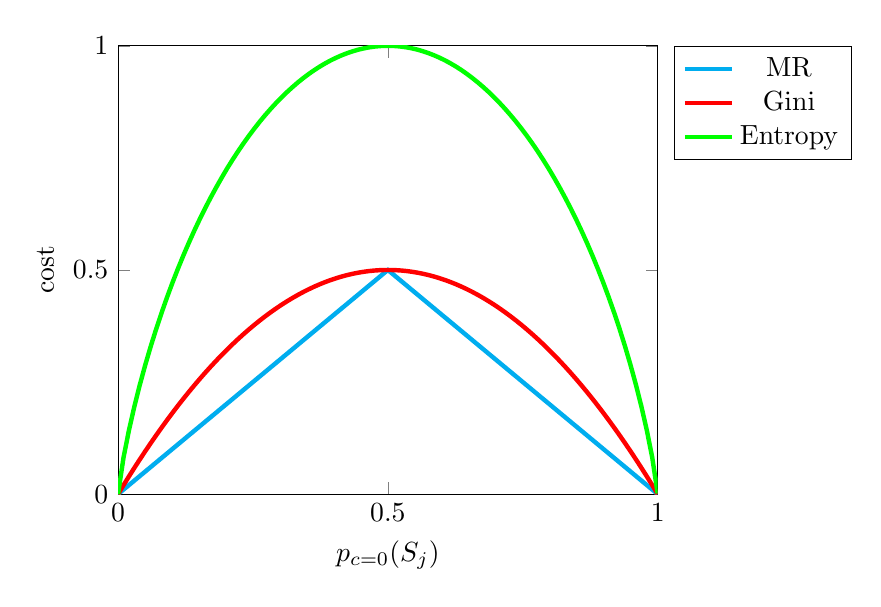
\begin{tikzpicture}
		\begin{axis} [
		xtick={0,0.5,1},
		ytick={0,0.5,1},
		xlabel={$p_{c=0}(S_j)$},
		ylabel={cost},
		xmin = 0, xmax = 1,
		ymin = 0, ymax = 1,
		samples = 100,
		legend pos=outer north east]
		\addplot [cyan, ultra thick, domain = 0:0.502,forget plot] {x};
		\addplot [cyan, ultra thick, domain = 0.498:1] {1-x};
		\addplot [red, ultra thick, domain = 0:1] {x*(1-x)+(1-x)*x};
		\addplot [green, ultra thick, domain = 0:1] {-x*log2(x)-(1-x)*log2(1-x)};
		\addlegendentry{MR}
		\addlegendentry{Gini}
		\addlegendentry{Entropy}
		\end{axis} 
	\end{tikzpicture}
\end{center}

\section{Overfitting}

Due to the complexity of the hypothesis class (there are $2^{2^D}$ possible Decision Trees with $D$ Boolean features, for example), overfitting can become an issue. One approach is limiting the maximum depth of the trees, but that can cause underfitting instead. Better approaches are the use of bagging or boosting instead.
\\\newline
A bagging technique specific to Random Forests (the name given to the ensemble of Decision Trees created with either bagging or boosting) is to pick split points (i.e. make decisions) randomly instead of optimally. Thus, $f^*$ and $t^*$ are instead picked as such
\[ j^* \sim U(\{1,\dots,D\}) = p(j) = \frac{1}{D} \]
\[ j^* \sim U(\mathcal{T}_f) = p(t) = \frac{1}{|\mathcal{T}_f|} \]

\end{document}

